
\chapter{Spécification des besoins}

\setcounter{page}{1}
\thispagestyle{empty}

\newpage

%================header and footer============

\fancyhf{}% Clear header/footer
\newpagestyle{ruled}
{\sethead{}{}{Spécifications des besoins}\headrule
  \setfoot{ISI : Institut Supérieur d'Informatique}{}
  { \thepage}\footrule}
\pagestyle{ruled}

\renewcommand\makeheadrule{\color{cyan}\rule[-.3\baselineskip]{\linewidth}{2.5pt}}
\renewcommand\makefootrule{\color{cyan}\rule[\baselineskip]{\linewidth}{2.5pt}}


%==============Début

 \section{Description du projet}
Le projet consiste à développer une application web pour la gestion des Allocations pour Voyages d'Affaires (AVA) destinée aux clients de la banque STB.
L'AVA permet aux clients de disposer d'une enveloppe de devises transférables destinée à couvrir les frais de vos voyages / séjours à l'étranger dans le cadre de leurs activités professionnelles.
L'application doit être sécurisée au niveau des échanges des messages et au niveau accès au contenu.
 
 \section{Identification des besoins fonctionnels}

Les besoins fonctionnels doivent répondre aux points précis du cahier des charges qui présente les exigences du futur outil en termes de fonctionnalités. Ce sont une sorte de contrat ou de promesse entre l'utilisateur et le développeur. Les fonctionnalités qui doivent être fournit par mon application sont les suivantes : 

\begin{itemize}
\item \textbf{L'accès et l'identification.}

\begin{itemize}
\item  L'application traite l'accès des utilisateurs.
\item Chaque utilisateur a une interface unique.
\end{itemize}



\item \textbf{Demande d'ouverture d'un dossier AVA.}

%========2eme liste integrée
\begin{itemize}
\item \textbf{Les types d'Allocation :}
L'Allocation pour Voyages d'Affaires peut prendre plusieurs formes :

%======3eme niveau
\begin{itemize}
\item A.V.A exportateur : 
Le montant de l'allocation est fixé actuellement à 25\% des recettes d'exportation de biens ou de services (Vente directe ou indirecte)
sans dépasser un plafond annuel de Cinq Cents Mille (500.000,000) dinars.

\item A.V.A importateur :
Le montant de l'allocation est déterminé à partir du montant des importations réalisées durant l'année précédente.\\
L'allocation est comprise entre 5000 et 50000 dinars.

\item A.V.A autres activités :

Le montant de l'allocation est déterminé à partir du montant du Chiffre d'affaires hors taxes déclaré de l'année précédente.\\
L'allocation est comprise entre 3000 et 30000 dinars.

\item A.V.A nouveau promoteur :
Le montant de l'allocation est fixé à Quinze Mille (15.000) dinars.\\
L'allocation est accordée une seule fois pour toute la période relative à la réalisation du projet.\\
Une fois le quota épuisé, le dossier est clôturé et le client peut choisir une autre catégorie d'AVA

\item A.V.A marchés réalisables à l'étranger :
Le montant de l'allocation est fixé à 15\% du prix du contrat de marché à titre duquel l'allocation est demandée .

\end{itemize} %3eme niveau
\end{itemize} %2eme niveau


Le client peut  demander à d'ouvrir un dossier AVA (Exportateur, Importateur, Autres Activités, Nouveau Promoteur, Marché réalisable à l'étranger) en remplissant un formulaire .

%=============Revenir au premiere liste==================
\item \textbf{Consulter l'avancement des dossiers AVA.}
Un dossier AVA a plusieurs états :
\item \textbf{Annulation de voyage.} 
Le client a le droit d'annuler sa voyage et de retourner l'argent dans le dossier AVA, dans un délai de 30 jours. 

\item \textbf{Rétrocession.} 
Après le retour du client d'une voyage d'affaire, il peut faire une rétrocession de l'argent restantes,dans un délai de 7 jours de son retour.
\item \textbf{Ajouter un Bénéficiaire.}
Les sociétés clientes du STB peuvent ajouter ses employés pour bénéficier de l'allocation.

\item \textbf{Désactiver un Bénéficiaire.}
Les sociétés clientes du STB peuvent désactiver un bénéficiaire pour qu'il ne bénéficie pas de l'allocation.

\end{itemize}
 
 \section{Identification des besoins non fonctionnels} 
 Outre que les besoins fonctionnels, il faut tenir compte des certains besoins non fonctionnels nécessaires pour une exploitation simple et consistantes des différentes fonctionnalités offertes :
 
 \begin{itemize}
 \item La rapidité de traitement : optimisation de temps de réponse s'approche le plus possible de temps réel.
 
 \item La convivialité : l'application doit être facile à utiliser. En effet, l'interface utilisateur doit être conviviale c'est-à-dire simple, ergonomique et facile à utiliser.
 
 \item L'ergonomie des interfaces hommes -machine (IHM) : l'ergonomie est définie comme l'ensemble des connaissances pour concevoir des applications qui puissent être utilisée avec le maximum d'efficacité et de sécurité. Notre application doit être d'une part utile (répond aux besoins utilisateurs) et d'une autre part utilisable (facile à utiliser).
 Pour ce fait, nous devons respecter les critères de qualité des interfaces.

\item Le système doit être une solution informatique performante dans la bonne circulation de l'information et du travail.
 
 \end{itemize}
 \section{Diagramme des cas d'utilisations global}
 
 \begin{figure}[!h]
\begin{center}

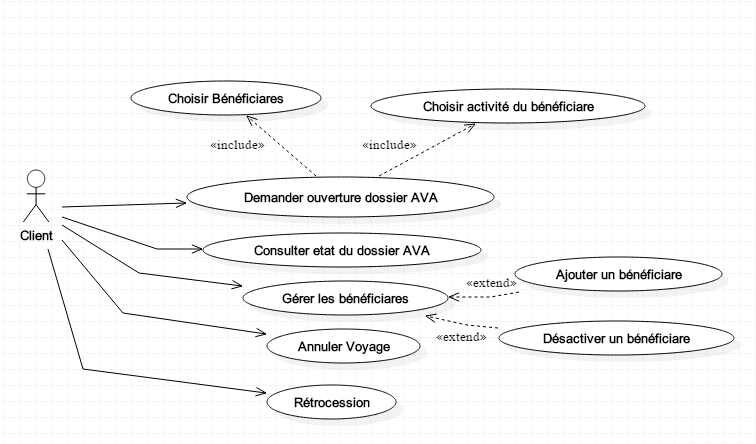
\includegraphics[width=10cm]{./conception/Global_use_case}

\caption{Diagramme des cas d'utilisations global}
\end{center}
\end{figure}

 
 \section{Identifications des acteurs et des cas d'utilisations}
 
 \subsection{Identification des acteurs}
 
 \subsection{Identification de cas d'utilisations}
 